\chapter{General Background}
\label{literature}

\section{Differential Analysis of Languages}

Language is a system that consists of the development, acquisition, maintenance and use of complex systems of communication, particularly the human ability to do so; and a language is any specific example of such a system. Estimates of the number of human languages in the world vary between 5,000 and 7,000. Languages as communication tools are different in many ways. Recall that when you first learn a second language (L2), the alphabet or words in that language looks so strange, especially for those languages using different sets of characters (for example Chinese and English). You may regard those words as a sequence of graphs without any meanings. Also, when you first listen to a sentence in the L2 or two people talking in L2, the sound waves are just noise to you. However, you are still aware that those sentences either in text or sound format are conveying specific information in a different way from your own language. How languages are different and where do those differences come from?

Language (or linguistic) typology is the science that studies ``similarities and differences among languages that do not stem from shared genetic relationship, language contact, or shared environmental conditions'' \citep{moravcsik_2012}. The goal of language typology is to describe and explain the common properties and structural diversity of the world's languages and how those properties generalize in cross-linguistic case \citep{bickel2001typology}. This discipline includes several subfields, depending on the ways languages are grouped into same class. An introductory categorization is provided in \citep{moravcsik2012introducing}:

\begin{enumerate}
\item Lexical typology: deals with characteristic ways in which language packages semantic material into words. For example, English uses different words for ``foot''/``leg'' and ``finger''/``toe'' while languages like Japanese and Russian use one word to represent ``foot''/``leg'' (``ashi'' in Japanese and ``noga'' in Russian) and ``finger''/``toe'' (``yubi'' in Japanese and ``palec'' in Russian).
\item Syntactic typology: deals with characteristic ways in which language packages words into sentences syntactically. For example, according to subject-verb-object positioning, languages can be grouped into different sets: SOV (such as French, German, Spanish and Chinese), SVO (such as English and Chinese) and so on, where the abbreviation represents the order of subject(S), verb(V) and object(O).
\item Morphological typology: deals with characteristics ways in which language forms words by combining morphemes. For example, morphological typology categorize languages into analytic languages and synthetic languages. Analytic languages, including Chinese and Vietnamese, contain very little inflection (inflection refers to ``the modification of a word to express different grammatical categories such as tense, case, voice, aspect, person, number, gender, and mood''), instead relying on features like word order and auxiliary words to convey meaning while synthetic languages, including most Indo-European languages, form words by affixing a given number of dependent morphemes to a root morpheme and word order is less important for synthetic languages.
\item Phonological typology: dealing with characteristics ways in which sounds are distributed across languages and phonological phenomena such as phoneme inventories, syllable structure, phonological alternations, stree/tone/intonation, prosodic morphology and so on. For example, in terms of consonant-vowel ratio, English has relatively is low and Russian is relatively high. In terms of syllable structure, English is relatively complex while Mandarin is relatively simple \citep{wals}.
\end{enumerate}

As introduced in Chapter \ref{introduction}, the current study focuses on phonological patterns of L1 and L2 and how they affect the phonological patterns of accented speech. The phonological difference among different languages will be introduced in this section. There are several data sources for language typology: UCLA Phonological Segment Inventory Database \citep{maddieson1992ucla}, Word Atlas of Language Structures (WALS) \citep{wals}, URIEL Typological Database \citep{littel2016uriel}, PHOIBLE \citep{phoible}, to name a few. Different databases have different data sources and language samples. Here, the features provided by WALS is used to illustrate the phonological difference among several languages for the reason that WALS provides simple ways to visualize and download the data. Those languages will be the target L1s in later sections of this dissertation.

\begin{figure}[h]
\centering
\captionsetup{justification=centering}
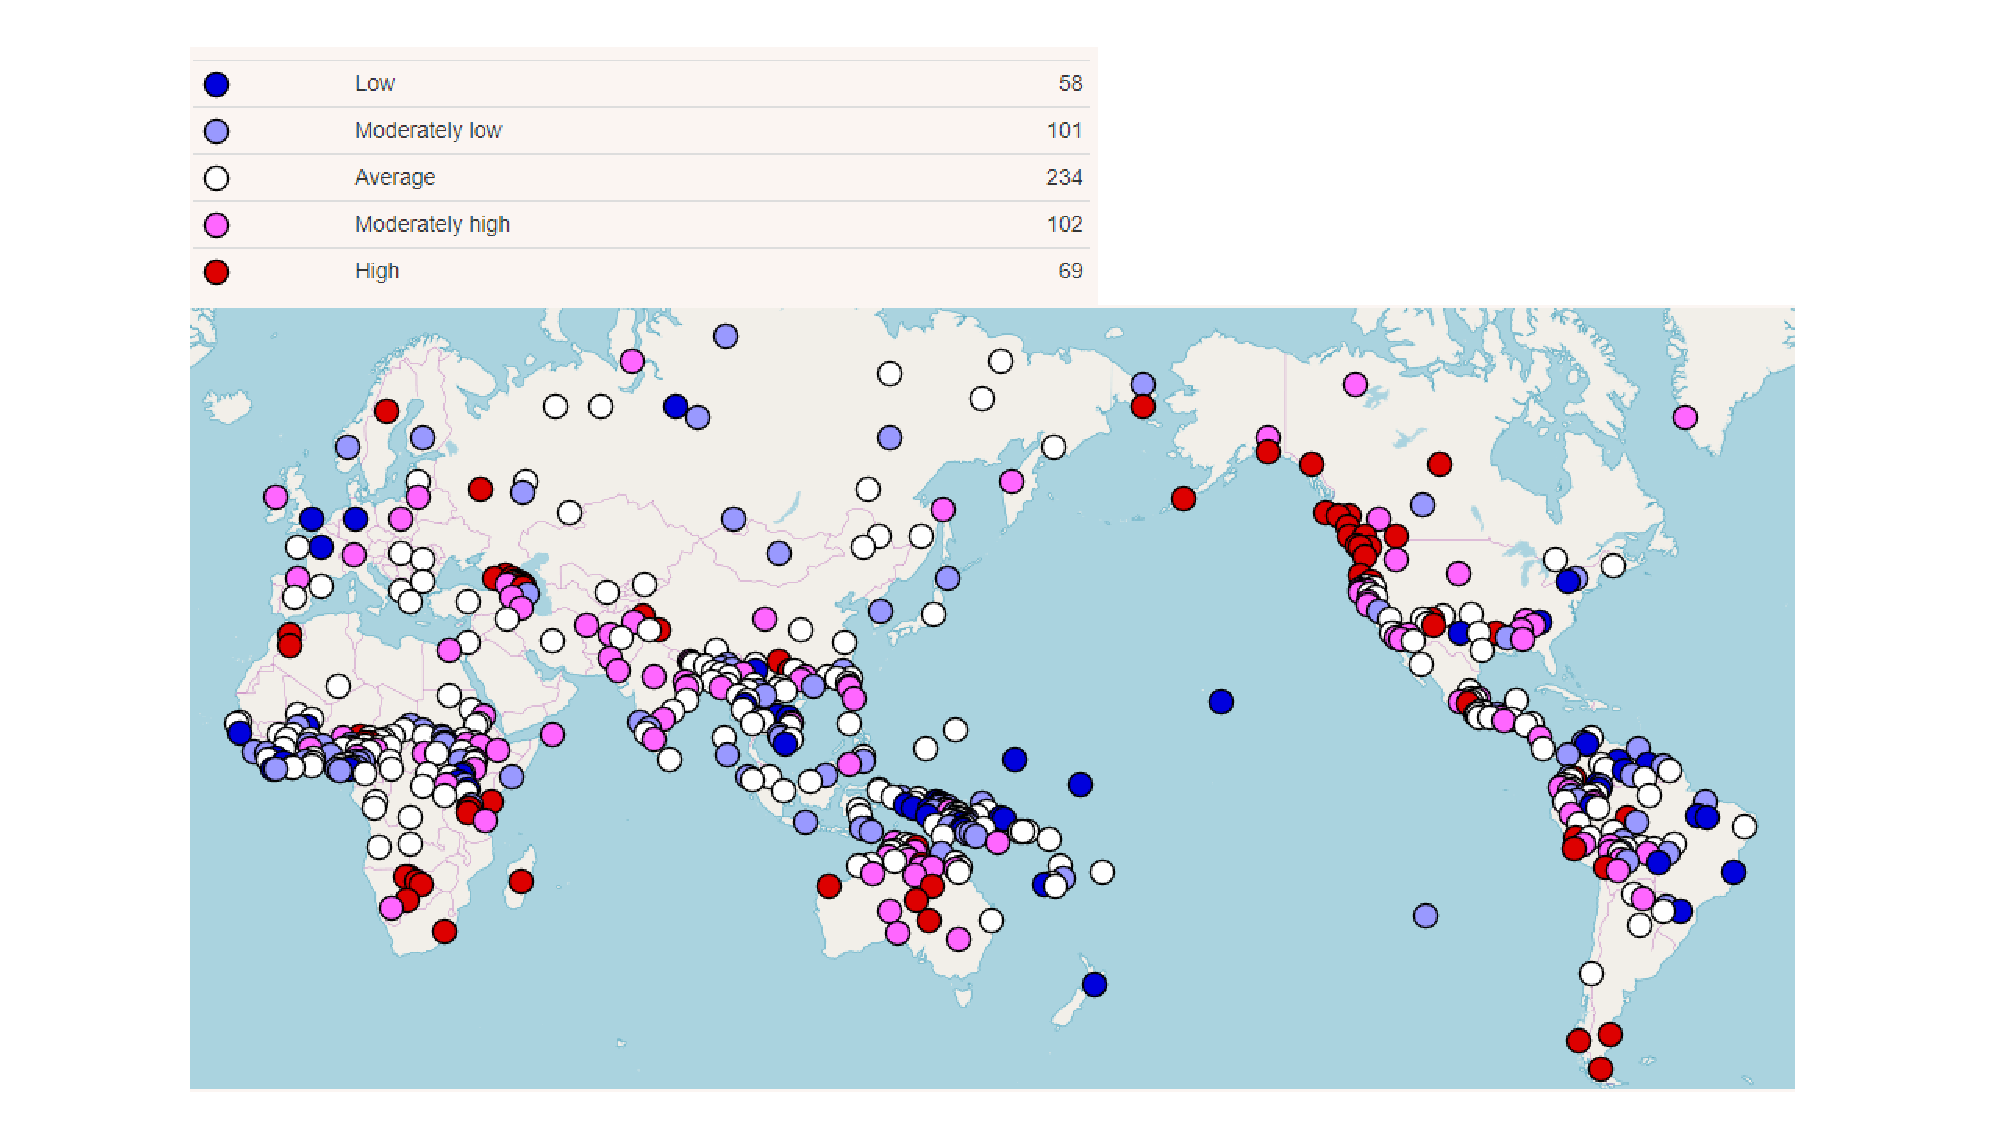
\includegraphics[width = 0.8\linewidth]{figures/WALS_example.pdf}
\caption{Consonant-vowel ratio across sampled languages by WALS. Different colors represent different level of consonant-vowel ratio: blue for low level, light blue for moderately low level, white for average level, magenta for moderately high level and red for high level.}
\label{fig:wals_example}
\end{figure}

First, in figure \ref{fig:wals_example}, the consonant-vowel ratio is used as an example of how phonological patterns are different across world's languages. Higher ratio means there are more consonants and less vowels in that language while lower ratio means the opposite. Take some commonly used languages as examples: English, German and French all have low ratio; Spanish, Persian and Mandarin have average ratio; Russian has high ratio.

\begin{table}[]
\centering
\caption{19 language phonological features summarized by WALS. The last column indicates whether the feature is phonetic or rhythmic feature. For detailed description of each feature, refer to \citep{wals}}
\label{table: wals_feature}
\begin{tabular}{|c|c|}
\hline
Feature name & Phonetic or Rhythmic \\ \hline
Consonant Inventories & Phonetic \\ \hline
Vowel Quality Inventories & Phonetic \\ \hline
Consonant-Vowel Ratio & Rhythmic\tablefootnote{Although Consonant-Vowel Ratio looks like a phonetic feature because it is the ratio of the number of consonants and vowels, most studies regard it as a rhythmic feature \citep{gil1986prosodic}.} \\ \hline
Voicing in Plosives and Fricatives & Phonetic \\ \hline
Voicing and Gaps in Plosive Systems & Phonetic \\ \hline
Uvular Consonants & Phonetic \\ \hline
Glottalized Consonants & Phonetic \\ \hline
Lateral Consonants & Phonetic \\ \hline
The Velar Nasal & Phonetic \\ \hline
Vowel Nasalization & Phonetic \\ \hline
Front Rounded Vowels & Phonetic \\ \hline
Syllable Structure & Rhythmic \\ \hline
Tone & Rhythmic \\ \hline
Fixed Stress Locations & Rhythmic \\ \hline
Weight-Sensitive Stress & Rhythmic \\ \hline
Weight Factors in Weight-Sensitive Stress System & Rhythmic \\ \hline
Rhythm Types & Rhythmic \\ \hline
Absence of Common Consonants & Phonetic \\ \hline
Presence of Uncommon Consonants & Phonetic \\ \hline
\end{tabular}
\end{table}

Next, it is clearer to do differential analysis of different languages with phonological patterns and to illustrate the distance among different languages on phonological feature space. To achieve this, several phonological features pre-summarized by WALS are selected. Based on whether there definitions are segmental or supra-segmental, those features are categorized into phonetic features and rhythmic features. Two groups of features represent language phonological patterns on phonetic space and rhythm space respectively. Table \ref{table: wals_feature} includes those features' names and indicates whether each feature is phonetic or rhythmic\footnote{Downloadable from \url{https://cdstar.shh.mpg.de/bitstreams/EAEA0-7269-77E5-3E10-0/wals_language.csv.zip}}. WALS assigns feature values to languages based on the structural properties of languages that describe one aspect of cross-linguistic diversity. For example, the feature ``Rhythm Types'' has five values: Trochaic (left-hand syllable in the foot is strong), Iambic (right-hand syllable in the foot is strong), Dual (system has both trochaic and iambic feet), Undetermined (no clear foot type) and Absent (no rhythmic stress). Those feature values are stored as a number, usually starting from 1, to represent each categories they belong to. To visualize those languages on a 2-dimensional space, the numeric values of each feature are used. If one feature is not applicable to a language, 0 is used instead. As a result, each language will have a 19-dimensional feature vector representing values of those features in table \ref{table: wals_feature}. Each feature vector is also split into phonetic and rhythmic feature vectors. Since each feature actually indicate a category, to make sure the distances among different categories are the same, one-hot encoding is used to convert the integer feature value to a vector consisting of 0s and 1s. The length of the encoded vector is equal to the number of categories that feature can be. For example, the ``Rhythm Types'' feature has 5 categories. Then, a number of 3 will be encoded as ``00010''. Multidimensional scaling (MDS), which seeks a low-dimensional representation of those feature vectors in which the distances respect well the distances in the original high-dimensional space, is employed to illustrate the 2-dimensional representation of each language in all phonological feature space (as shown in figure \ref{fig:all_mds}), phonetic feature only space (as shown in figure \ref{fig:phonetic_mds}) and rhythmic feature only space (as shown in \ref{fig:rhythmic_mds}) with the encoded language features.

\begin{figure}[!htb]
\centering
\minipage{0.55\textwidth}
  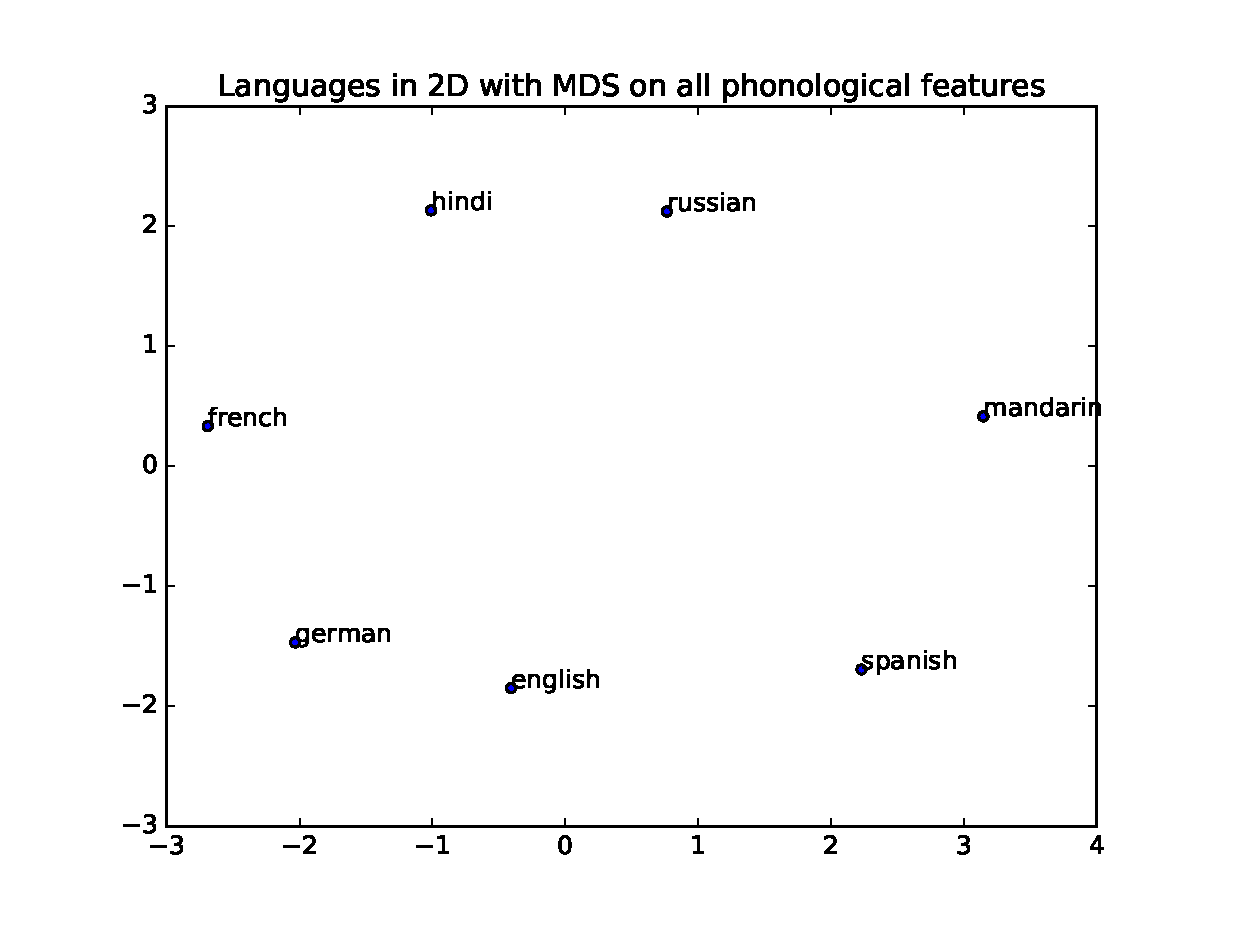
\includegraphics[width=\linewidth]{figures/all_MDS.eps}
  \caption{2D visualization of all features with MDS.}\label{fig:all_mds}
\endminipage\hfill
\\
\minipage{0.55\textwidth}
  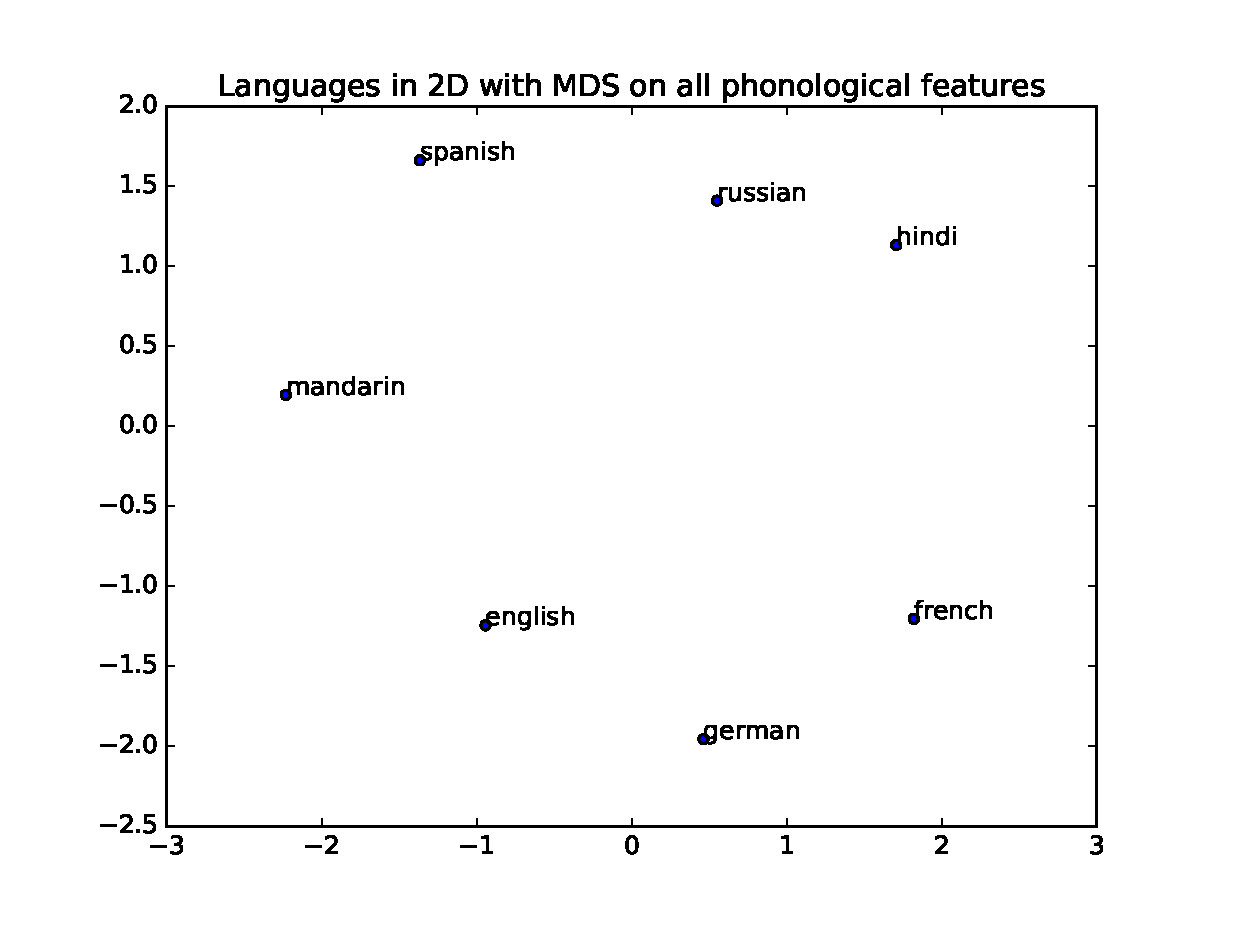
\includegraphics[width=\linewidth]{figures/phono_MDS_wals.eps}
  \caption{2D visualization of phonetic only features with MDS.}\label{fig:phonetic_mds}
\endminipage\hfill
\\
\minipage{0.55\textwidth}%
  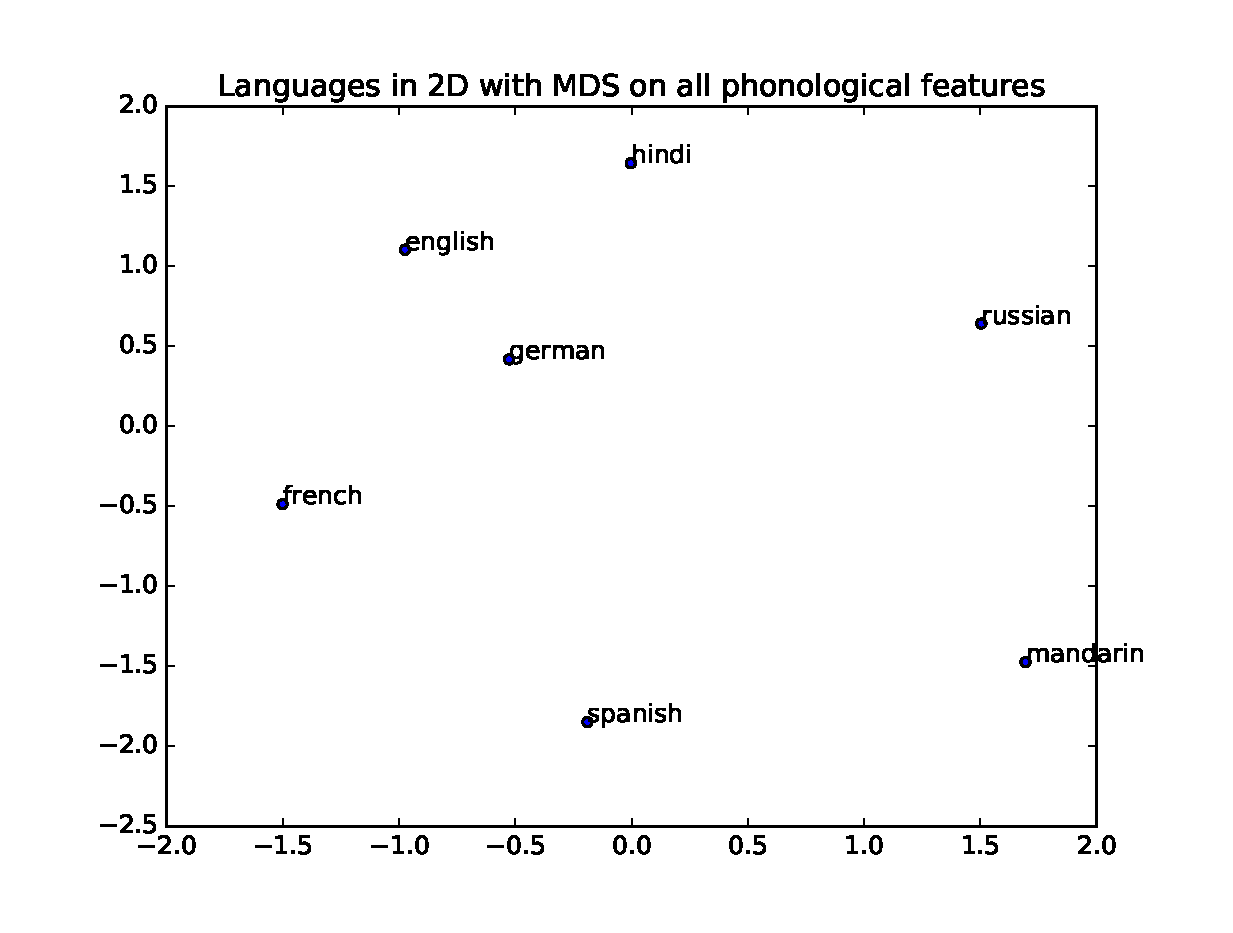
\includegraphics[width=\linewidth]{figures/rhythmic_MDS.eps}
  \caption{2D visualization of rhythmic only features with MDS.}\label{fig:rhythmic_mds}
\endminipage
\end{figure}

Along with the 2-dimensional visualization, normalized pair-wise distance matrices are also shown in table \ref{table:conf_all} for all features, table \ref{table:conf_phonetic} for phonetic features and table \ref{table:conf_rhythmic} fir rhythmic features. The pairwise distance between two languages is calculated as follows: count the number of different values for corresponding dimensions of the feature vectors of two languages without one-hot encoding. This will result in a $N \times N$ matrix where N is the number of languages; normalize the matrix by the maximum value in the matrix. From the feature visualization and normalized pair-wise distance matrices, it can be found that English, German and French are relatively close to each other on all three feature space while other languages are relative far from those three languages. If English is regarded as L2, German is closest to English on all features space. Furthermore, German is closer to English on rhythmic space than phonetic space. So is French. However, Mandarin and Spanish are closer to English on phonetic space than rhythmic space. One important question this study wants to investigate is that whether those L1 to L2 distance patterns will manifest in the accented speech perception: how the relative importance of segmental features and supra-segmental features relates to the distance to L2 on phonetic and rhythmic space.

\begin{table}[!htb]
\centering
\caption{Normalized pairwise distance on all features space.}
\label{table:conf_all}
\resizebox{0.55\columnwidth}{!}{%
\begin{tabular}{|c|c|c|c|c|c|c|c|}
\hline
 & German & Spanish & French & Russian & Hindi & English & Mandarin \\ \hline
German & 0 & 0.92 & 0.33 & 0.67 & 0.67 & 0.33 & 0.83 \\ \hline
Spanish &  & 0 & 0.83 & 0.67 & 0.75 & 0.67 & 0.50 \\ \hline
French &  &  & 0 & 0.67 & 0.58 & 0.58 & 1.00 \\ \hline
Russian &  &  &  & 0 & 0.42 & 0.58 & 0.75 \\ \hline
Hindi &  &  &  &  & 0 & 0.50 & 0.92 \\ \hline
English &  &  &  &  &  & 0 & 0.83 \\ \hline
Mandarin &  &  &  &  &  &  & 0 \\ \hline
\end{tabular}}
\end{table}

\begin{table}[!htb]
\centering
\caption{Normalized pairwise distance on rhythmic features only space.}
\label{table:conf_phonetic}
\resizebox{0.55\columnwidth}{!}{%
\begin{tabular}{|c|c|c|c|c|c|c|c|}
\hline
 & German & Spanish & French & Russian & Hindi & English & Mandarin \\ \hline
German & 0 & 1.00 & 0.29 & 0.71 & 0.86 & 0.43 & 0.71 \\ \hline
Spanish &  & 0 & 1.00 & 0.57 & 0.71 & 0.57 & 0.43 \\ \hline
French &  &  & 0 & 0.71 & 0.57 & 0.71 & 1.00 \\ \hline
Russian &  &  &  & 0 & 0.29 & 0.57 & 0.71 \\ \hline
Hindi &  &  &  &  & 0 & 0.71 & 0.86 \\ \hline
English &  &  &  &  &  & 0 & 0.71 \\ \hline
Mandarin &  &  &  &  &  &  & 0 \\ \hline
\end{tabular}}
\end{table}

\begin{table}[!htb]
\centering
\caption{Normalized pairwise distance on rhythmic features only space.}
\label{table:conf_rhythmic}
\resizebox{0.55\columnwidth}{!}{%
\begin{tabular}{|c|c|c|c|c|c|c|c|}
\hline
 & German & Spanish & French & Russian & Hindi & English & Mandarin \\ \hline
German & 0 & 0.80 & 0.40 & 0.60 & 0.40 & 0.20 & 1.00 \\ \hline
Spanish &  & 0 & 0.60 & 0.80 & 0.80 & 0.80 & 0.60 \\ \hline
French &  &  & 0 & 0.60 & 0.60 & 0.40 & 1.00 \\ \hline
Russian &  &  &  & 0 & 0.60 & 0.60 & 0.80 \\ \hline
Hindi &  &  &  &  & 0 & 0.20 & 1.00 \\ \hline
English &  &  &  &  &  & 0 & 1.00 \\ \hline
Mandarin &  &  &  &  &  &  & 0 \\ \hline
\end{tabular}}
\end{table}

The previous features are summarized by linguistics on a high systematic level. How those features manifest themselves in the acoustic recordings of different languages? How the languages' differences manifest themselves in the key parameters of acoustic speech signal including intensity, pitch, formants, envelop and so on? Several studies have investigate this and those findings. An early study \citep{parmenter1933experimental} compared the acoustic characteristics between English and French reading speech and showed that pitch is more important as an element of accent than intensity for French speech while intensity is more important for English speech. Also, French speech has more pitch variation than English. Studies in \citep{jongman1989acoustic,bradlow1995comparative,al2005does} investigated the relationship between vowel inventories and vowel space (defined as the two-dimensional area bounded by lines connecting first and second formant frequency coordinates of vowels) and concluded that vowel space depends on the size of vowel inventory: the larger the inventory, the bigger the acoustic space. The work by \citep{wagner2003voice} showed that predominant factors in voice quality are different across different languages. In terms of speech rhythm, an influential study in \citep{ramus1999correlates} studied the representation of linguistic speech rhythm in acoustic speech signal. Several acoustic measurements for speech rhythm are proposed to discriminate the rhythm classes of different languages. Those measurements include the percentage of vocalic segment in an utterance ($\%V$), the standard deviation of consonant intervals ($\Delta C$) and the standard deviation of vowel intervals ($\Delta V$). Figure is taken from \citep{ramus1999correlates} to show how $\%V$ and $\Delta C$ can discriminate languages. Based this study, other measurements like variational coefficient of consonant/vowel intervals \citep{dellwo2006rhythm}, pairwise variability index of consonant/vowel intervals \citep{grabe2002durational} are also proposed. Those studies that correlate those linguistically summarized phonological language features with acoustic measurements lay the foundation of the methodology used in this study.

\begin{figure}[h]
\centering
\captionsetup{justification=centering}
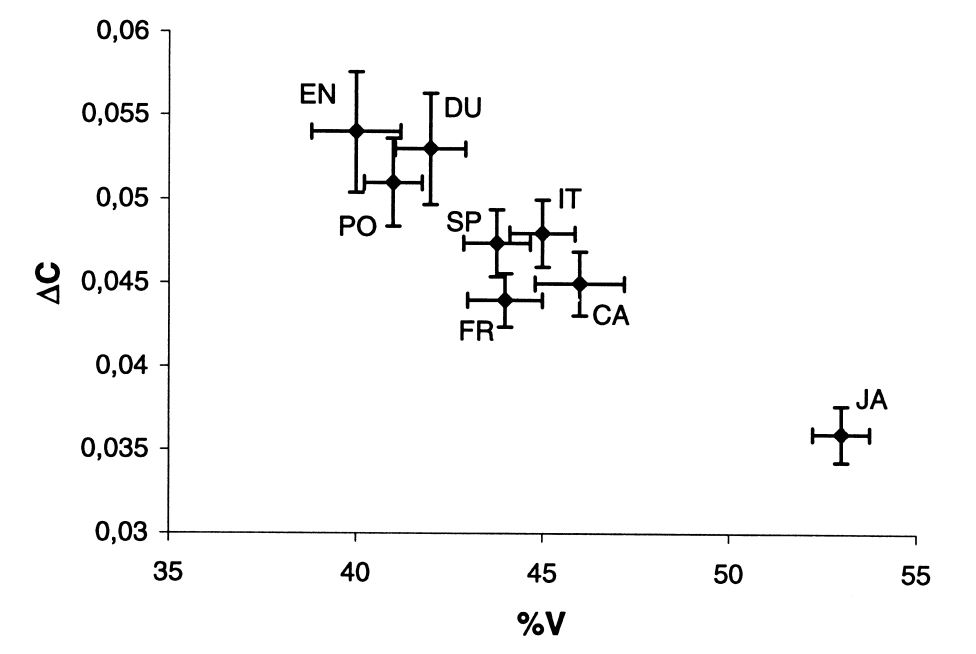
\includegraphics[width = 0.8\linewidth]{figures/ramus_paper.JPG}
\caption{Distribution of languages over the ($\%V$, $\Delta C$) plane. EN: English, PO: Polish, DU: Dutch, SP: Spanish, IT: Italian, FR: French, CA: Catalan, JA: Japanese.}
\label{fig:wals_example}
\end{figure}
